%%%%%%%%%%%%%%%%%%%%%%%%%%%%%%%%%%%%%%%%%%%
%
% From a template maintained at https://github.com/jamesrobertlloyd/cbl-tikz-poster
%
%%%%%%%%%%%%%%%%%%%%%%%%%%%%%%%%%%%%%%%%%%%


\documentclass[portrait,a0b,final,a4resizeable]{include/a0poster}


\usepackage{multicol}
\usepackage{color}
\usepackage{morefloats}
\usepackage[pdftex]{graphicx}
\usepackage{rotating}
\usepackage{amsmath, amsthm, amssymb, bm}
\usepackage{array}
\usepackage{booktabs}
\usepackage{multirow}
\usepackage{hyperref}
\usepackage{include/picins}
\usepackage{tikz}
\usetikzlibrary{shapes.geometric,arrows,chains,matrix,positioning,scopes,calc}
\tikzstyle{mybox} = [draw=white, rectangle]
\definecolor{darkblue}{rgb}{0,0.08,0.45}
\definecolor{blue}{rgb}{0,0,1}
\usepackage{dsfont}
\usepackage[margin=0.5in]{geometry}
\usepackage{fp}

%%%%%%%%%%%%%%%%%%%%%%%%%%%%%%%%%%%%%%%%%%%
%
% myfig
%
% \myfig - replacement for \figure
% necessary, since in multicol-environment 
% \figure won't work        
%                 
%%%%%%%%%%%%%%%%%%%%%%%%%%%%%%%%%%%%%%%%%%%

\newcommand{\myfig}[3][0]{
\begin{center}
  \vspace{1.5cm}
  \includegraphics[width=#3\hsize,angle=#1]{#2}
  \nobreak\medskip
\end{center}}

%%%%%%%%%%%%%%%%%%%%%%%%%%%%%%%%%%%%%%%%%%%
%
% mycaption                
%
% \mycaption - replacement for \caption
% necessary, since in multicol-environment \figure and
% therefore \caption won't work
%
%%%%%%%%%%%%%%%%%%%%%%%%%%%%%%%%%%%%%%%%%%%

%\newcounter{figure}
\setcounter{figure}{1}
\newcommand{\mycaption}[1]{
  \vspace{0.5cm}
  \begin{quote}
    {{\sc Figure} \arabic{figure}: #1}
  \end{quote}
  \vspace{1cm}
  \stepcounter{figure}
}

%%%%%%%%%%%%%%%%%%%%%%%%%%%%%%%%%%%%%%%%%%%
%
% Some standard colours
%
%%%%%%%%%%%%%%%%%%%%%%%%%%%%%%%%%%%%%%%%%%%

\definecolor{camlightblue}{rgb}{0.601 , 0.8, 1}
\definecolor{camdarkblue}{rgb}{0, 0.203, 0.402}
\definecolor{camred}{rgb}{1, 0.203, 0}
\definecolor{camyellow}{rgb}{1, 0.8, 0}
\definecolor{lightblue}{rgb}{0, 0, 0.80}
\definecolor{white}{rgb}{1, 1, 1}
\definecolor{whiteblue}{rgb}{0.80, 0.80, 1}

%%%%%%%%%%%%%%%%%%%%%%%%%%%%%%%%%%%%%%%%%%%
%
% Some look and feel definitions
%
%%%%%%%%%%%%%%%%%%%%%%%%%%%%%%%%%%%%%%%%%%%

\setlength{\columnsep}{0.03\textwidth}
\setlength{\columnseprule}{0.0018\textwidth}
\setlength{\parindent}{0.0cm}

%%%%%%%%%%%%%%%%%%%%%%%%%%%%%%%%%%%%%%%%%%%
%
% \mysection - replacement for \section*
% 
% Puts a pretty box around some text
% TODO - any other thoughts for what this box should look like
%
%%%%%%%%%%%%%%%%%%%%%%%%%%%%%%%%%%%%%%%%%%%

\tikzstyle{mysection} = [rectangle, 
			draw=none, 
			shade, 
			outer color=camlightblue!30,
			inner color=camlightblue!30,
			text width=0.965\columnwidth,
			text centered,
			rounded corners=20pt,
			minimum height=0.09\columnwidth]

\newcommand{\mysection}[1]
{
\begin{center}
  \begin{tikzpicture}
    \node[mysection] {\sffamily\bfseries\LARGE#1};
  \end{tikzpicture}
\end{center}
}

%%%%%%%%%%%%%%%%%%%%%%%%%%%%%%%%%%%%%%%%%%%
%
% Set the font
%
% TODO - Not sure what a canonical choice is - feel free to modify
%
%%%%%%%%%%%%%%%%%%%%%%%%%%%%%%%%%%%%%%%%%%%

\renewcommand{\familydefault}{cmss}
\sffamily

%%%%%%%%%%%%%%%%%%%%%%%%%%%%%%%%%%%%%%%%%%%%%%%%%%%%
%%%               Background                     %%%
%%%%%%%%%%%%%%%%%%%%%%%%%%%%%%%%%%%%%%%%%%%%%%%%%%%%

\newcommand{\background}[3]{
  %\definecolor{cgradbegin}{#1}
  %\definecolor{cgradend}{#2}
 % \psframe[fillstyle=gradient,gradend=cgradend,
 % gradbegin=cgradbegin,gradmidpoint=#3](0.,0.)(1.\textwidth,-1.\textheight)
}




%%%%%%%%%%%%%%%%%%%%%%%%%%%%%%%%%%%%%%%%%%%%%%%%%%%%
%%%                pcolumn                       %%%
%%%%%%%%%%%%%%%%%%%%%%%%%%%%%%%%%%%%%%%%%%%%%%%%%%%%

\newenvironment{pcolumn}[1]{
  \begin{minipage}{#1\textwidth}
  \begin{center}
}{
  \end{center}
  \end{minipage}
}



%%%%%%%%%%%%%%%%%%%%%%%%%%%%%%%%%%%%%%%%%%%%%%%%%%%%
%%%                pbox                          %%%
%%%%%%%%%%%%%%%%%%%%%%%%%%%%%%%%%%%%%%%%%%%%%%%%%%%%

\definecolor{lcolor}{rgb}{0, 0, 0.80}
\definecolor{gcolor1}{rgb}{1, 1, 1}
\definecolor{gcolor2}{rgb}{.80, .80, 1}

  % \def\fc{fillcolor}
  % \def\getfc #1=#2\par{\def\ffc{#1} \ifx\ffc\fc #2\fi} 
  % \def\getfillcolor #1,#2\par{\getfc #1\par \getfc #2\par}

 %  \newcommand{\psshadowbox}[2]{%[2][magenta]{
%      \fbox{Input arg: #1}
%      \fbox{#1} 
%      \fbox {\getfillcolor #1\par}
%      \def\col{\getfillcolor #1\par}
 
%      \let\coll=\col
%       \coll
 %     \colorbox{\col}{#2}
%       \mbox
   %   \coloredshadowbox{black}{\coll}{#2}
%   }

\newcommand{\pbox}[4]{
%\psshadowbox[#3]{
%\fbox{
\mbox{
\begin{minipage}[t][#2][t]{#1}
#4
\end{minipage}
}%}
}

%%%%%%%%%%%%%%%%%%%%%%%%%%%%%%%%%%%%%%%%%%%
%
% Poster environment
%
% Centres everything and can be used to define the width of the content
%
%%%%%%%%%%%%%%%%%%%%%%%%%%%%%%%%%%%%%%%%%%%

\newenvironment{poster}{
  \begin{center}
  \begin{minipage}[c]{\textwidth}
}{
  \end{minipage}
  \end{center}
}

\def\newarrow{\mbox{\begin{tikzpicture}
             \useasboundingbox{(-3pt,-4.5pt) rectangle (19pt,1pt)};
             \draw[->] (0,-0.07)--(17pt,-0.07);\end{tikzpicture}}}



\usepackage{include/preamble}


% Custom notation
\newcommand{\fdeep}{\vf^{(1:L)}}
\newcommand{\flast}{\vf^{(L)}}
\newcommand{\Jx}{J_{\vx \rightarrow \vy}}
\newcommand{\Jxx}{J_{\vx \rightarrow \vy}(\vx)}
\newcommand{\Jy}{J_{\vy \rightarrow \vx}}
\newcommand{\Jyy}{J_{\vy \rightarrow \vx}(\vy)}
\newcommand{\detJyy}{ \left| J_{\vy \rightarrow \vx}(\vy) \right|}

\newcommand\transpose{{\textrm{\tiny{\sf{T}}}}}
\newcommand{\note}[1]{}
\newcommand{\hlinespace}{~\vspace*{-0.15cm}~\\\hline\\\vspace*{0.15cm}}
\newcommand{\embeddingletter}{g}
\newcommand{\bo}{{\sc bo}}
\newcommand{\agp}{Arc \gp}

\newcommand{\D}{\mathcal{D}}
\newcommand{\X}{\mathbf{X}}
\newcommand{\y}{y}
\newcommand{\data} {\X, \y}
\newcommand{\x}{\mathbf{x}}
\newcommand{\f}{\mathit{f}}

\newcommand{\fx}{ f(\mathbf{x}) }
\newcommand{\U}{\mathcal{U}}
\newcommand{\E}{\mathbf{E}}

\def\layersep{10cm}
\def\nodesep{6cm}
\def\nodesize{4cm}

\newcommand{\numdims}[0]{2}
\newcommand{\numhidden}[0]{2}
\newcommand{\upnodedist}[0]{3cm}
\newcommand{\bardist}[0]{\hspace{-0.2cm}}

\newcommand{\neuronfunc}[2]{
\FPeval{\result}{clip(#1+#2)}
\includegraphics[width=5.5cm]{../../figures/two-d-draws/sqexp-draw-\result}}

\newlength{\arrowsize}  
\pgfarrowsdeclare{biggertip}{biggertip}{  
  \setlength{\arrowsize}{10pt}  
  \addtolength{\arrowsize}{2\pgflinewidth}  
  \pgfarrowsrightextend{0}  
  \pgfarrowsleftextend{-5\arrowsize}  
}{  
  \setlength{\arrowsize}{1pt}  
  \addtolength{\arrowsize}{\pgflinewidth}  
  \pgfpathmoveto{\pgfpoint{-5\arrowsize}{4\arrowsize}}  
  \pgfpathlineto{\pgfpointorigin}  
  \pgfpathlineto{\pgfpoint{-5\arrowsize}{-4\arrowsize}}  
  \pgfusepathqstroke  
} 


% Custom commmands.

\def\jointspacing{\vspace{0.3in}}

\def\boxwidth{0.21\columnwidth}
\newcommand{\gpdrawbox}[1]{
\setlength\fboxsep{0pt}
\hspace{-0.36in} 
\fbox{\hspace{-4mm}
\includegraphics[width=\boxwidth]{../figures/deep_draws/deep_gp_sample_layer_#1}
\hspace{-4mm}}}

\newcommand{\mappic}[1]{\hspace{-0.05in}\includegraphics[width=\boxwidth]{../../figures/seed-0-map/latent_coord_map_layer_#1}}
 
\newcommand{\mappiccon}[1]{\hspace{-0.05in}\includegraphics[width=\boxwidth]{../../figures/seed-0-map-connected/latent_coord_map_layer_#1}}

\newcommand{\spectrumpic}[1]{
\includegraphics[trim=4.5mm 0mm 4mm 3mm, clip, width=0.44\columnwidth]{../figures/spectrum/layer-#1}} 

\newcommand{\feat}{\vh}





\begin{document}
\begin{poster}
\vspace{1\baselineskip}   % Add some space at the top of the poster


%%% Header
\begin{center}
\begin{pcolumn}{1.03}

\newcommand{\logowidth}{0.09\textwidth}
\pbox{0.99\textwidth}{}{linewidth=2mm,framearc=0.3,linecolor=camdarkblue,fillstyle=gradient,gradangle=0,gradbegin=white,gradend=white,gradmidpoint=1.0,framesep=1em}{
%
%%% Cambridge Logo
\raisebox{-0cm}{
\begin{minipage}[c]{\logowidth}
  \begin{center}
    
\includegraphics[width=6cm]{badges/University_Crest}
    \vspace{.1in}
    
\includegraphics[width=6cm]{badges/unicamtext.pdf}
  \end{center}
\end{minipage}}
%
%%% Title
\begin{minipage}[c][9cm][c]{0.76\textwidth}
  \begin{center}
    {\sffamily \VeryHuge \textbf{Avoiding Pathologies in Very Deep Networks}}\\[10mm]
    {\huge\sffamily \Huge David Duvenaud, Oren Rippel, Ryan P. Adams, Zoubin Ghahramani\\[7.5mm]
     }
  \end{center}
\end{minipage}
%
% Harvard logo
\raisebox{-0cm}{
\begin{minipage}[c]{\logowidth}
  \begin{flushright}
    
\includegraphics[width=8cm,trim=2em 0em 2em 2em, clip]{badges/harvard}
  \end{flushright}
\end{minipage}}
%
}
\end{pcolumn}
\end{center}

\vspace*{3cm}

\large


%%%%%%%%%%%%%%%%%%%%%%%%%%%%%%%%%%%%%%%%%%%%%%%%%%%%%%%%%%%%%%%%%%%%%%
%%% Beginning of Document
%%%%%%%%%%%%%%%%%%%%%%%%%%%%%%%%%%%%%%%%%%%%%%%%%%%%%%%%%%%%%%%%%%%%%%

\Large

\begin{multicols}{2}


\mysection{Abstract}

\vspace*{-1.5cm}
\null\hspace*{3cm}\begin{minipage}[c]{0.8\columnwidth}
\centering
\begin{itemize}
\item We compare architectures by building priors over deep nets.
\item We characterize a pathology in standard architectures.
\item We show a simple alternative architecture that fixes the problem.
\end{itemize}
\end{minipage}

\jointspacing

\mysection{Nonparametric priors on deep neural networks}

\center
\begin{centering}

\def\layersep{8cm}
\def\nodesep{3.3cm}
\def\halfshift{1.65cm}
\def\nodesize{2.5cm}

\newcommand{\numdims}[0]{3}
\newcommand{\numhidden}[0]{4}
\newcommand{\upnodedist}[0]{2.3cm}

\newcommand{\neuronfunc}[2]{
\FPeval{\result}{clip(#1+#2)}
%
\null\hspace*{-0.5cm}\includegraphics[width=1.9cm, clip, trim=10mm 0mm 10mm 0mm]{../../figures/two-d-draws/sqexp-draw-\result}
%\end{pgfonlayer}
}


\begin{tabular}{c}
\begin{tikzpicture}[draw=black, node distance=\layersep]
    \tikzstyle{interarrows}=[->, ultra thick, -biggertip, black!50, line width = 2pt, shorten >= -0cm, shorten <= -0cm]
    \tikzstyle{neuron}=[circle, draw = black, inner sep=-0pt, line width = 2pt]
    \tikzstyle{input neuron}=[neuron, minimum size=\nodesize];
    \tikzstyle{output neuron}=[neuron, minimum size=\nodesize];
    \tikzstyle{hidden neuron}=[neuron, minimum size=\nodesize];
    \tikzstyle{annot} = [text width=4em, text centered]

    % Draw the input layer nodes
    \foreach \name / \y in {1,...,\numdims}
        \node[input neuron] (I-\name) at (0,-\nodesep*\y) {$x_\y$};

    % Draw the hidden layer nodes
    \foreach \name / \y in {1,...,\numhidden}
        \path[yshift=\halfshift] node[hidden neuron] (H-\name) at (\layersep,-\nodesep*\y) { \neuronfunc{\y}{0}};

    % Draw the hidden layer nodes
    \foreach \name / \y in {1,...,\numhidden}
        \path[yshift=\halfshift] node[hidden neuron] (H2-\name) at (2*\layersep,-\nodesep*\y) {\neuronfunc{\y}{4}};

    % Draw the output layer node
    \foreach \name / \y in {1,...,\numdims}
    	\node[output neuron] (O-\name) at (3*\layersep,-\nodesep*\y) {\neuronfunc{\y}{8}};

    % Connect every node in the input layer with every node in the hidden layer.
    \foreach \source in {1,...,\numdims}
        \foreach \dest in {1,...,\numhidden}
            \path (I-\source) edge[interarrows] (H-\dest);
            
    \foreach \source in {1,...,\numhidden}
        \foreach \dest in {1,...,\numhidden}
            \path (H-\source) edge[interarrows] (H2-\dest);            

    % Connect every node in the hidden layer with the output layer
    \foreach \source in {1,...,\numhidden}
        \foreach \dest in {1,...,\numdims}
    	    \path (H2-\source) edge[interarrows] (O-\dest);

    % Annotate the layers
    \node[annot,above of=I-1, node distance=\upnodedist] {Inputs};
    \node[annot,below of=I-\numdims, node distance=\upnodedist] {$\vx$};    
    \node[annot,above of=H-1, node distance=\upnodedist, text width = 7cm] {Hidden Layer};
    \node[annot,above of=H2-1, node distance=\upnodedist, text width = 7cm] {Hidden Layer};
    \node[annot,below of=H-\numhidden, node distance=2.5cm, text width = 7cm] {$\vf^{(1)}(\vx)$};
    \node[annot,below of=H2-\numhidden, node distance=2.5cm, text width = 7cm] {$\vf^{(2)}(\vf^{(1)}(\vx))$};
    \node[annot,above of=O-1, node distance=\upnodedist] {Outputs};
    \node[annot,below of=O-\numdims, node distance=2.5cm, text width = 7cm] {$\vy$};
\end{tikzpicture}
\end{tabular}



\end{centering}


Deep \gp{}s are compositions of functions, each $f^{(\ell)} \simind \GPt{0}{k(\vx, \vx')}$. 
\begin{align*}
\vf^{(1:L)}(\vx) = \vf^{(L)}(\vf^{(L-1)}(\dots \vf^{(2)}(\vf^{(1)}(\vx)) \dots))
\end{align*}

\vspace{0.5in} 
 
\mysection{Random deep nets capture few degrees of freedom}



A density warped by a deep-\gp{} distributed function:
\vspace{0.5in}

\centering
\renewcommand{\tabcolsep}{0.5cm}
%\extracolsep{1cm}
\begin{tabular}{cccc}
Identity Map & 1 Layer & 4 Layers & 6 Layers \\
\gpdrawbox{1} & \gpdrawbox{2} & \gpdrawbox{4} & \gpdrawbox{6} \\
$p(\vx)$ & $p(\vf^{(1)}(\vx))$ & $p(\vf^{(1:4)}(\vx))$ &  $p(\vf^{(1:6)}(\vx))$
\end{tabular}

\jointspacing

As depth increases, density concentrates along one-dimensional filaments.

\jointspacing\jointspacing\jointspacing


Sampled mappings illustrate properties of this prior on functions:
\jointspacing

\centering
\begin{tabular}{cccc}
Identity Map & 1 Layer & 2 Layers & 40 Layers \\
\hspace{-0.1in}
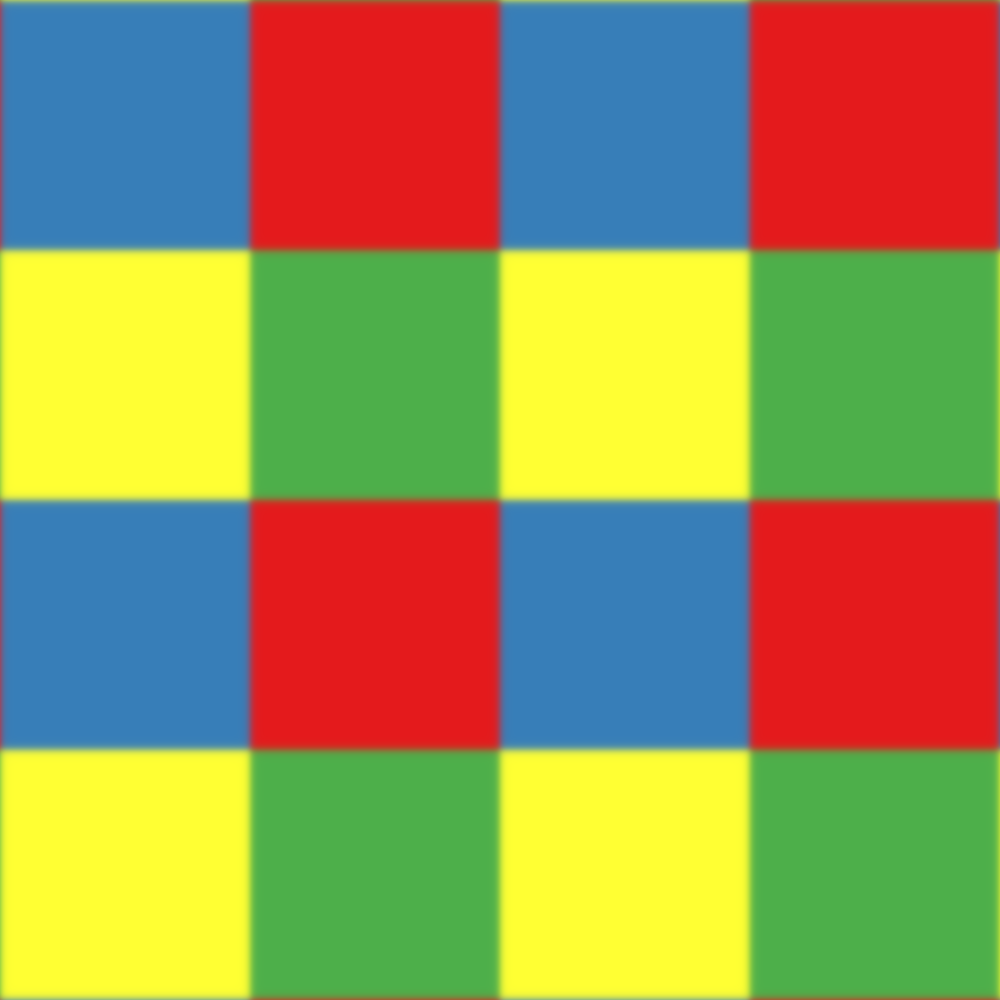
\includegraphics[width=\boxwidth]{../../figures/seed-0-map/layer_0} & \mappic{1} & \mappic{10} & \mappic{40} \\
$\vy = \vx$ & $\vy = \vf^{(1)}(\vx)$ & $\vy = \vf^{(1:2)}(\vx)$ & $\vy = \vf^{(1:40)}(\vx)$
\end{tabular}

\jointspacing

As depth increases, there is usually only one direction we can move $\vx$ to change $\vy$.







\newpage



\mysection{Good representations change along all tangents}
\jointspacing

\begin{tabular}{cc}
\begin{minipage}[c]{0.45\columnwidth}
\centering
\begin{tabular}{c}
Contours of representation \\
%\includegraphics[width=0.45\columnwidth]{figures/hidden_good} &
\begin{tikzpicture}[pile/.style={line width = 3pt, ->, >=stealth'}]
    \node[anchor=south west,inner sep=0] at (0,0) {
    	\includegraphics[clip, trim = 0cm 12cm 0cm 0.0cm, width=\columnwidth]{../figures/hidden_good}
    };
    \coordinate (D) at (2.7,2.35);
    \coordinate (Do) at (4.3,0.9);
    \coordinate (Dt) at (5,5);
    
    \draw[pile] (D) -- (Dt) node[above, text width=5em] { tangent };
    \draw[pile] (D) -- (Do) node[right, text width=5em] { orthogonal };
\end{tikzpicture}
\end{tabular}

\end{minipage}
&
\begin{minipage}[c]{0.5\columnwidth}
Representation $\vy = \vf(\vx)$ must change in directions tangent to the data manifold, to preserve information. { \color{mydarkblue} (Rifai et. al., 2011)}
\end{minipage}
\end{tabular}

\jointspacing






\mysection{Explaining the pathology}




\begin{tabular}{cc}
\begin{minipage}[c]{0.4\columnwidth}

\begin{itemize}
\item The Jacobian of a deep \gp{} is a product of independent Gaussian matrices.
\item Singular value spectrum shows relative size of derivatives.
\item As the net deepens, the derivative in one direction becomes much larger than all the others.
\end{itemize}

\end{minipage}
&
\begin{minipage}[c]{0.55\columnwidth}
\begin{centering}
\begin{tabular}{cc}
2 layer spectrum & 6 layer spectrum \\
\hspace{-0.16in} \spectrumpic{2} &
\hspace{-0.16in} \spectrumpic{6} \\
Singular values & Singular values  
%2 layers & 4 layers & 6 layers
\end{tabular}
\end{centering}
\end{minipage}
\end{tabular}






\jointspacing
\jointspacing

\mysection{Fixing the pathology}
\centering
\begin{itemize}
	\item Following {\color{mydarkblue} Neal, (1995)} we connect the input to every layer:
\end{itemize}

\jointspacing

%\def\layersep{1.33cm}
\def\nodeseptwo{1.8cm}
%\def\nodesize{.35cm}

%\newcommand{\numdims}[0]{3}
%\newcommand{\numhidden}[0]{4}
%\newcommand{\upnodedist}[0]{0.6cm}
%\newcommand{\bardist}[0]{\hspace{-0.2cm}}

\begin{tabular}{c}
\bardist
Standard architecture: \\
\begin{tikzpicture}[draw=black!80]
    \tikzstyle{neuron}=[circle,minimum size=17pt, draw = black!80, fill = white, thick]
    \tikzstyle{input neuron}=[neuron, fill=green!50];
    \tikzstyle{output neuron}=[neuron, fill=red!50];
    \tikzstyle{hidden neuron}=[neuron, fill=blue!50];
    \tikzstyle{pile} =[thick, ->, >=stealth', shorten <=7pt, shorten >=8pt];

    % Define the input layer node
    \coordinate (I) at (0, 0);


    % Define the hidden layer nodes
    \foreach \name / \i in {1,...,\numhidden}
    {
        \coordinate (H-\name) at (\nodeseptwo * \i, 0);
    }

    % Connect every node            
    \foreach \name in {1,...,\numhidden}
    {
	 \path[pile] (I) edge (H-\name) {};
         %\path[pile] (I) edge [bend left] (H-\name) {};
    }

    \draw (I) node[neuron] {};
    \draw (I) node[below = 0.5cm]  {$\vx$};

    % Draw the hidden layer nodes
    \foreach \name / \y in {1,...,\numhidden}
    {
	\draw (H-\name) node[neuron]  {};
        \draw (H-\name) node[below = 0.34cm] {$\vf^{(\y)}(\vx)$};
    }
\end{tikzpicture} \\
\vspace{\baselineskip}
\\
Input-connected architecture: \\
\bardist
\begin{tikzpicture}[draw=black!80]
    \tikzstyle{neuron}=[circle,minimum size=17pt, draw = black!80, fill = white, thick]
    \tikzstyle{input neuron}=[neuron, fill=green!50];
    \tikzstyle{output neuron}=[neuron, fill=red!50];
    \tikzstyle{hidden neuron}=[neuron, fill=blue!50];
    \tikzstyle{pile} =[thick, ->, >=stealth', shorten <=7pt, shorten >=8pt];

    % Define the input layer node
    \coordinate (I) at (0, 0);


    % Define the hidden layer nodes
    \foreach \name / \y in {1,...,\numhidden}
    {
        \coordinate (H-\name) at (\nodeseptwo*\y, 0);
    }

    % Connect every node            
    \path[pile] (I) edge (H-1) {};
    \foreach \name in {2,...,\numhidden}
    {
	 \path[pile] (I) edge (H-\name) {};
         \path[pile] (I) edge [bend left] (H-\name) {};
    }

    \draw (I) node[neuron] {};
    \draw (I) node[below = 0.5cm]  {$\vx$};

    % Draw the hidden layer nodes
    \foreach \name / \y in {1,...,\numhidden}
    {
	\draw (H-\name) node[neuron]  {};
        \draw (H-\name) node[below = 0.34cm] {$\vf^{(\y)}(\vx)$};
    }
\end{tikzpicture} 
\end{tabular}

\jointspacing

\newcommand{\gpdrawboxcon}[1]{
\setlength\fboxsep{0pt}
\hspace{-0.4in} 
\fbox{
\includegraphics[width=0.47\columnwidth]{../../figures/connected_deep_sample_seed_0/deep_sample_connected_layer#1}
}}

\begin{tabular}{cc}
\begin{minipage}[c]{0.4\columnwidth}
Pathology is now resolved in deep density models:
Density does not concentrate along filaments when the input connects to all layers.
\end{minipage}
&
\begin{minipage}[c]{0.45\columnwidth}
\centering
\begin{tabular}{cc}
%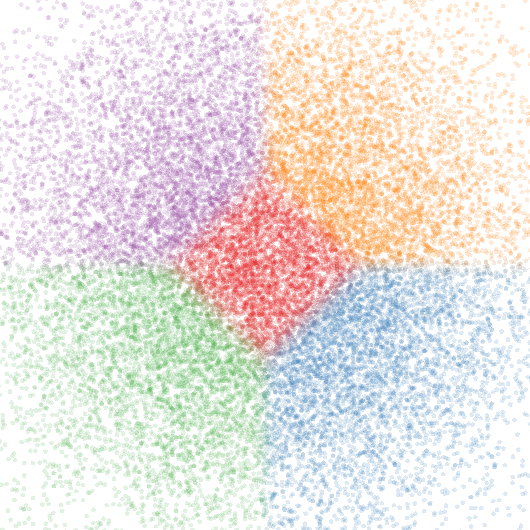
\includegraphics[width=0.3\columnwidth]{figures/deep_draws/deep_gp_sample_layer_1} &
%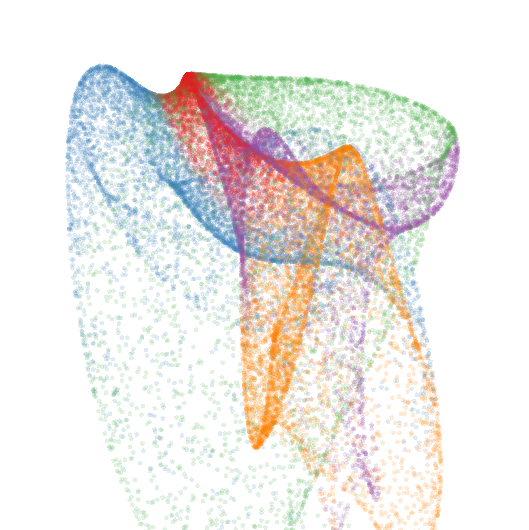
\includegraphics[width=0.3\columnwidth]{figures/deep_draws_connected/deep_sample_connected_layer2} &
%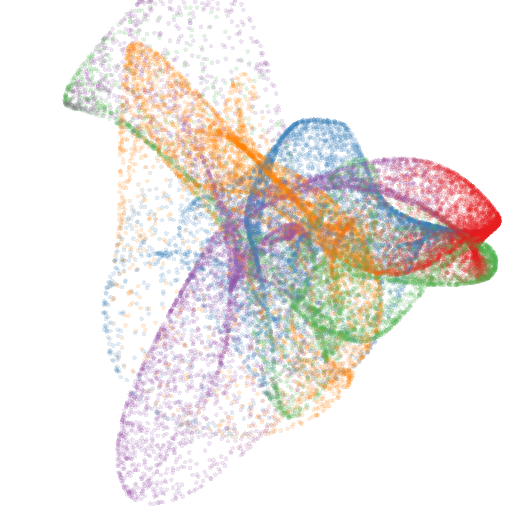
\includegraphics[width=0.3\columnwidth]{figures/deep_draws_connected/deep_sample_connected_layer3} \\
%$p(\vx)$ & $p(f_1(\vx))$ & $p(f_2(f_1(\vx), \vx))$ \\ \\
%\gpdrawboxcon{2} &
 4 Layers & 5 Layers \\
\gpdrawboxcon{4} &
\gpdrawboxcon{5}
\end{tabular}
\end{minipage}
\end{tabular}

\jointspacing
\jointspacing

\vspace{0.3in}

\begin{tabular}{cccc}
Identity Map %$\vy = \vx$ 
& 2 Layers & 10 Layers & 40 Layers \\%\\2 Layers: $\vy = f_1(f_2(\vx))$ \\
\hspace{-0.5in} \hspace{-0.05in}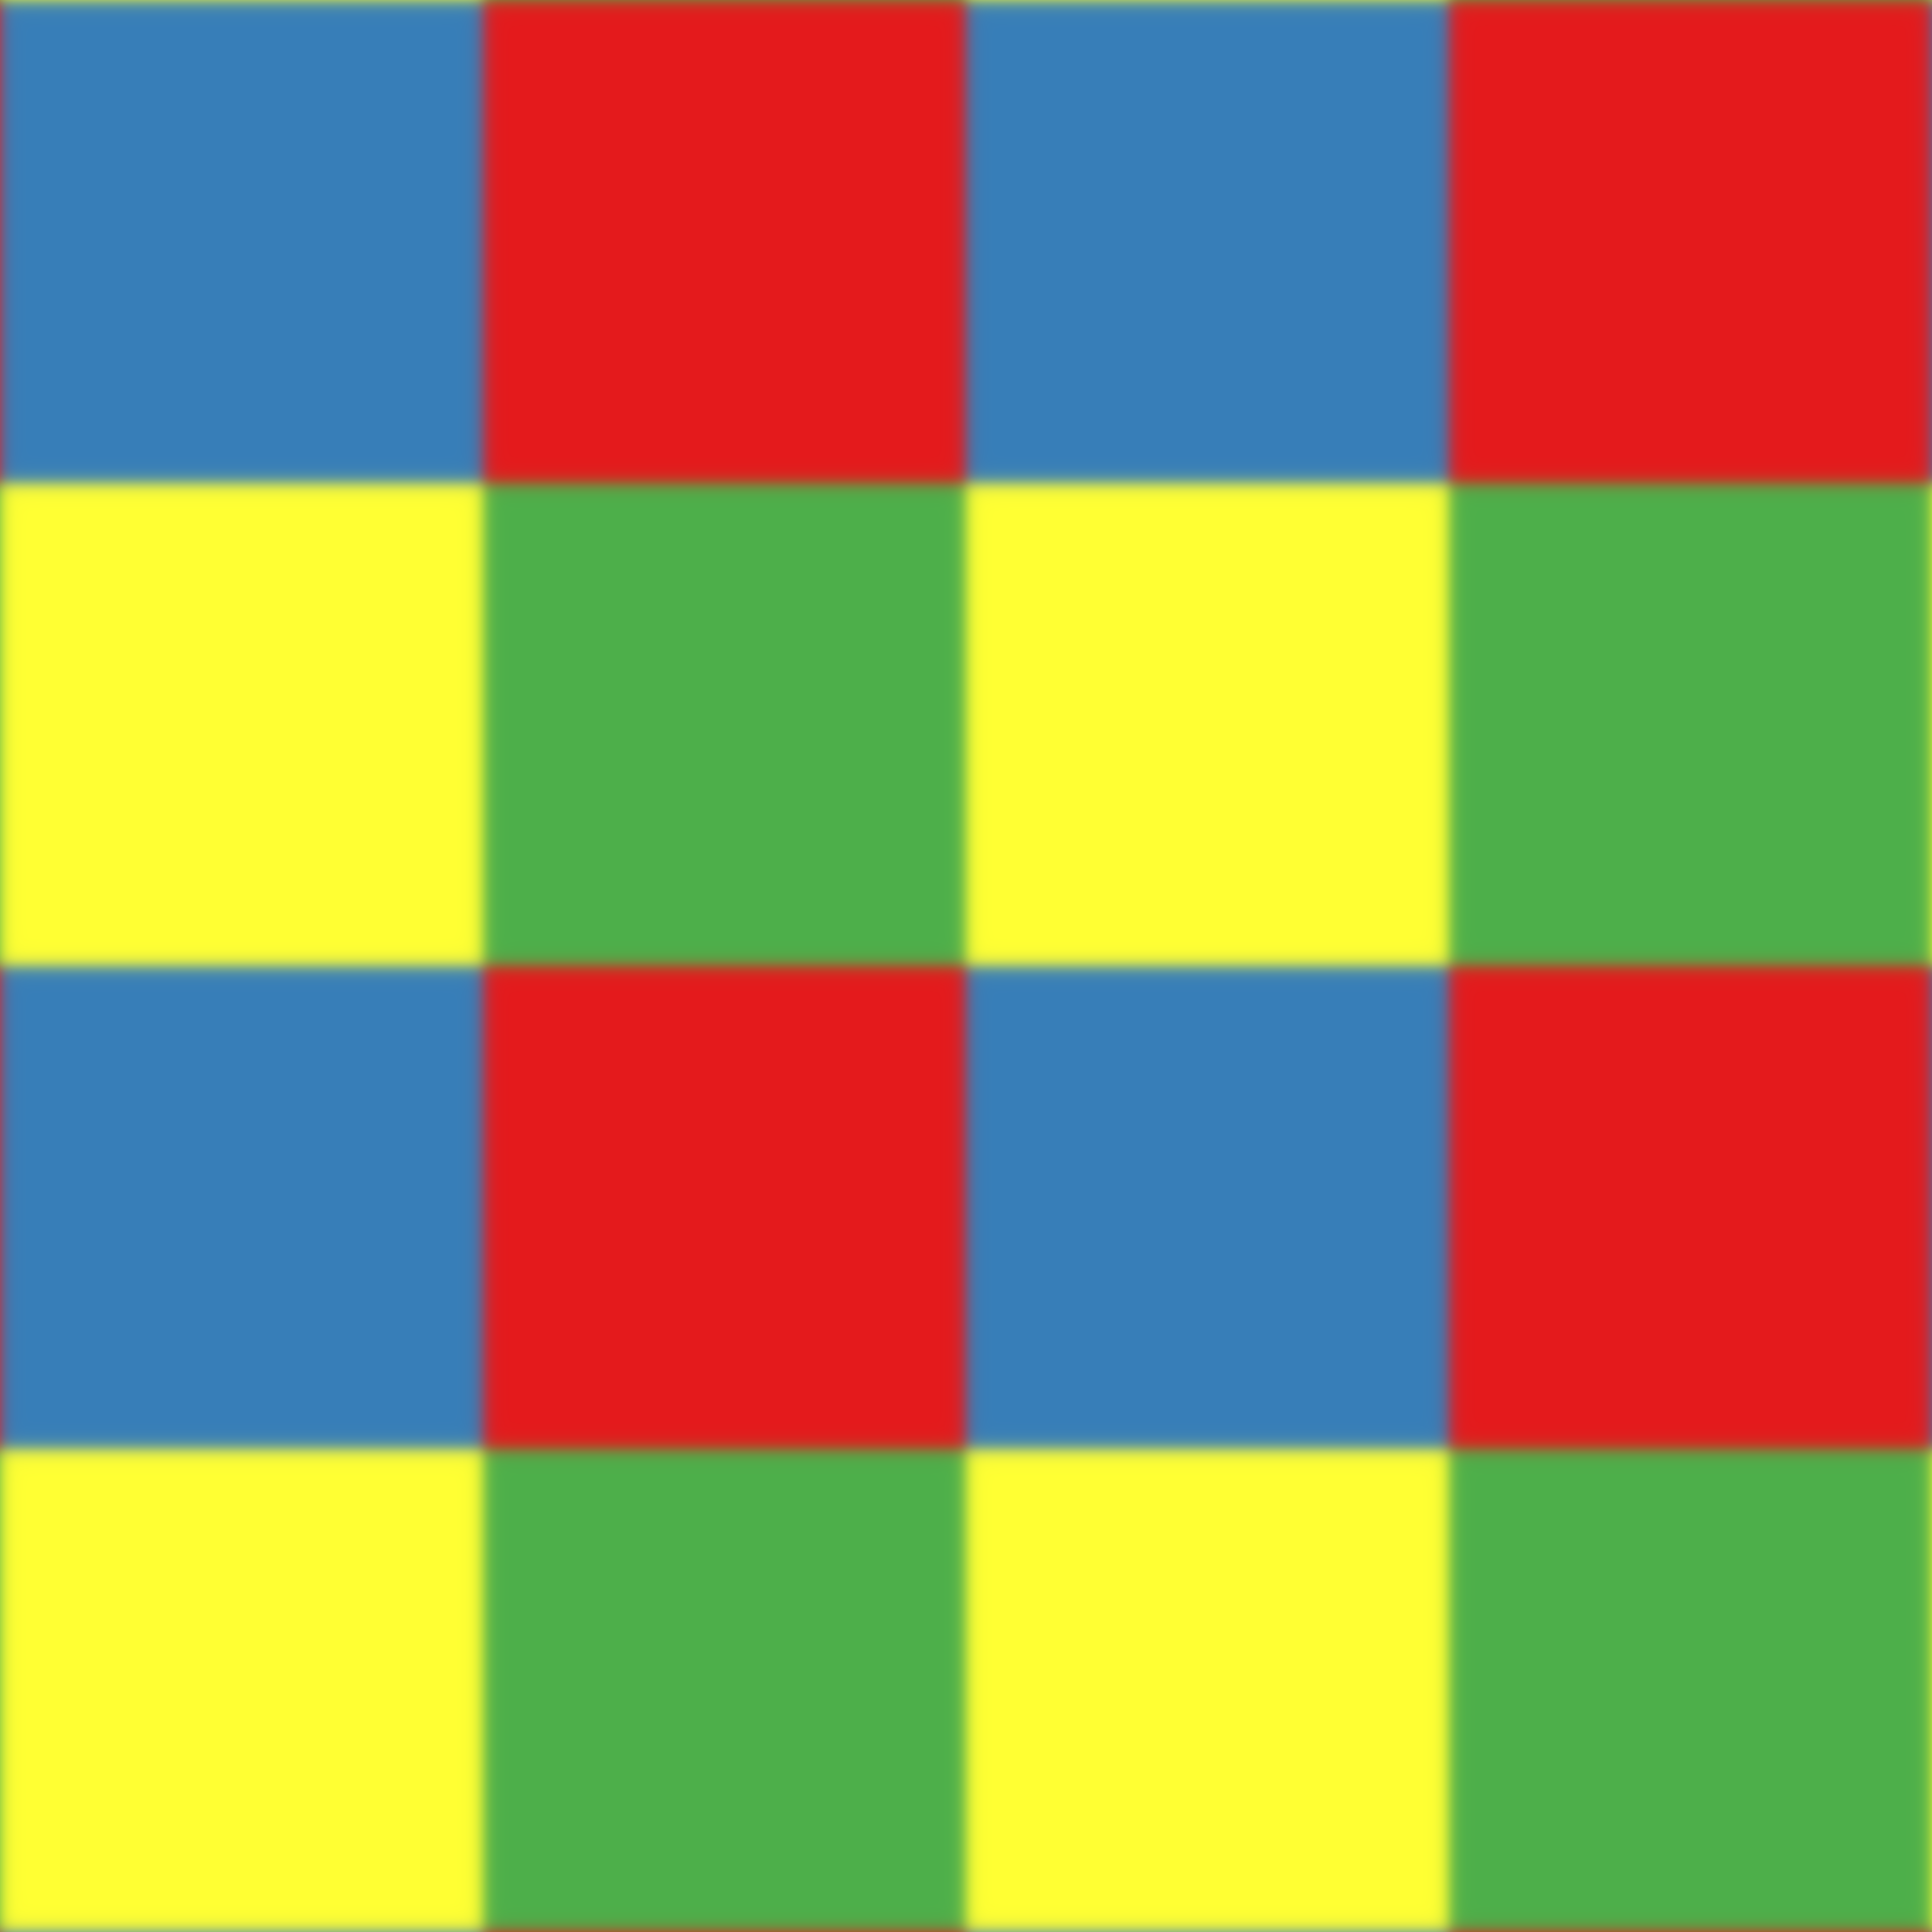
\includegraphics[width=\boxwidth]{../../figures/seed-0-map-connected/layer_0} & \mappiccon{2} & \mappiccon{10} & \mappiccon{40}
%\mappic{4} & \mappic{10} & \mappic{40} \\
%4 Layers & 10 Layers & 
\end{tabular}

\jointspacing
Locally up to $D$ degrees of freedom, at any depth.





%\mysection{Conclusions}


%\raggedright

%\begin{tabular}{cc}
%\begin{minipage}[c]{0.8\columnwidth}

%\begin{itemize}
%	\item Random networks capture fewer degrees of freedom as they get deeper
%	\item Connecting the input to each layer resolves this pathology
%\end{itemize}


%\end{minipage}
%&
%\begin{minipage}[c]{0.2\columnwidth}
%\begin{centering}
%
\includegraphics[width=\linewidth]{figures/qrcode-paper-link}
%\end{centering}
%\end{minipage}
%\end{tabular}
%
%
%

\end{multicols}


\vspace*{3cm}

\begin{center}
\begin{pcolumn}{1.03}

\pbox{0.99\textwidth}{}%{linewidth=2mm,framearc=0.3,linecolor=camdarkblue,fillstyle=gradient,gradangle=0,gradbegin=white,gradend=white,gradmidpoint=1.0,framesep=1em}
{}
{
%\begin{minipage}[c][9cm][c]{\textwidth}
  \begin{center}
    {\sffamily \VeryHuge \textbf{Other Results}}
  \end{center}
%\end{minipage}
}
\end{pcolumn}
\end{center}




\begin{multicols}{2}


\mysection{Dropout in Gaussian processes}

\begin{tabular}{cc}
\begin{minipage}[c]{0.65\columnwidth}
\begin{itemize}
\item One-layer GPs are infinitely-wide neural nets
\item Dropping out features has no effect
\item Dropping out inputs gives mixture of GPs
\item This mixture has closed-form covariance $$\covarianceargs{}{f(\vx'), f(\vx)} = \frac{1}{2^D} \sum_{\vr \in \{0,1\}^D}  \prod_{d=1}^D k_d(\vx_d, \vx_d')^{r_d}$$
\end{itemize}
\end{minipage}
&
\begin{minipage}[c]{0.3\columnwidth}
\centering
\begin{tabular}{c}
\null\hspace*{-0.2in} 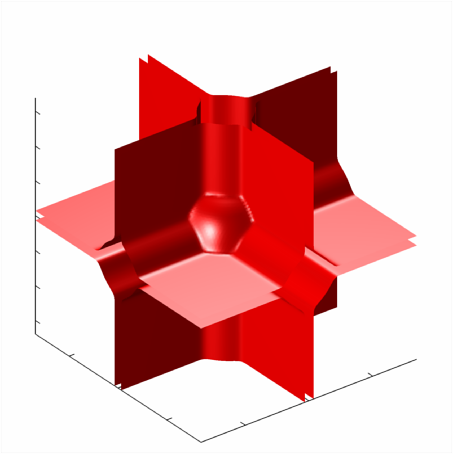
\includegraphics[trim=0em 0em 0em 0em, clip, width=0.9\columnwidth]{figures/3d-kernel/3d_add_kernel_321}\\
Dropout covariance \\isocontour
\end{tabular}
\end{minipage}
\end{tabular}



\mysection{Infinitely deep kernels}
\vspace*{-1cm}
\begin{minipage}[c]{0.6\columnwidth}
\begin{itemize}
%\item Can also analyze fixed deep feature mappings:
%\item {\color{mydarkblue} (Cho, 2012) } built kernels from multiple layers of feature mappings:
\item Kernels correspond to feature mappings:
$${k_1(\vx, \vx') = \feat(\vx) \tra \feat(\vx')}$$
\item Can compose feature maps to get deep kernels:
$${k_2(\vx, \vx') = \feat(\feat(\vx)) \tra \feat(\feat(\vx'))}$$
\item Closed form for arbitrarily deep kernels.
\end{itemize}

Code at {\color{mydarkblue}{\texttt{github.com/duvenaud/deep-limits}}}\\
Paper at {\color{mydarkblue}{\texttt{arxiv.org/abs/1402.5836}}}

\end{minipage}
\begin{minipage}[c]{0.39\columnwidth}
\begin{centering}
\begin{tabular}{c}
%\hspace{-0.5cm}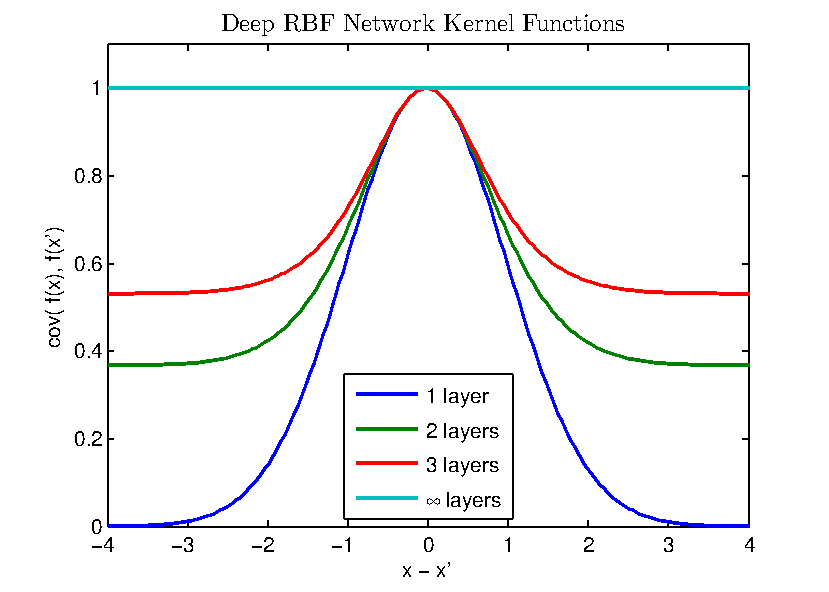
\includegraphics[width=0.33\columnwidth, clip, trim = 0cm 0cm 1cm 0.61cm]{../figures/deep_kernel} &
Deep connected kernel \\
$k_\infty(\vx, \vx') = $ \\ $\log \left(k_\infty(\vx, \vx) \right) + 1 + \frac{1}{2} || \vx - \vx' ||_2^2$ \\[0.5cm]
\hspace{-0.5cm}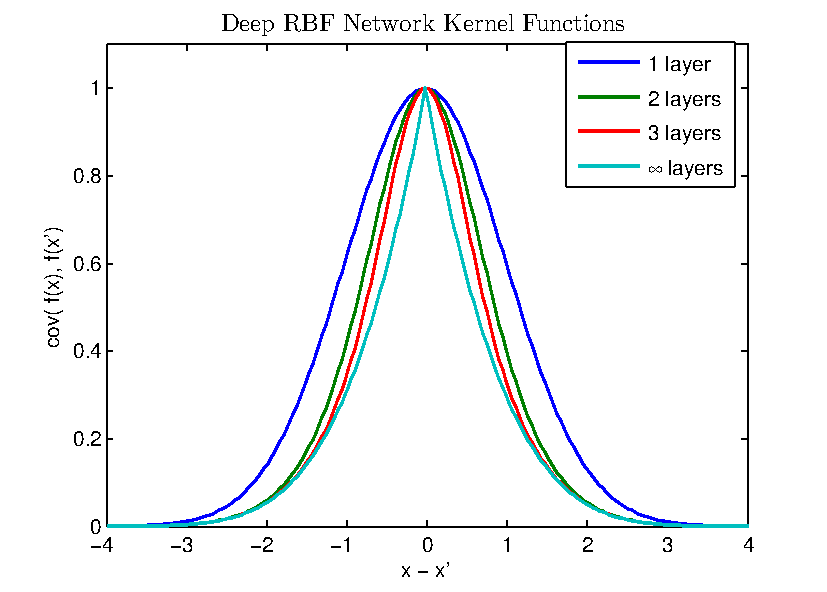
\includegraphics[width=\columnwidth, clip, trim = 0cm 0.4cm 0.9cm 0.3cm]{../figures/deep_kernel_connected} \\
$x - x'$
%Connected \gp{} draws \\
%\hspace{-0.5cm}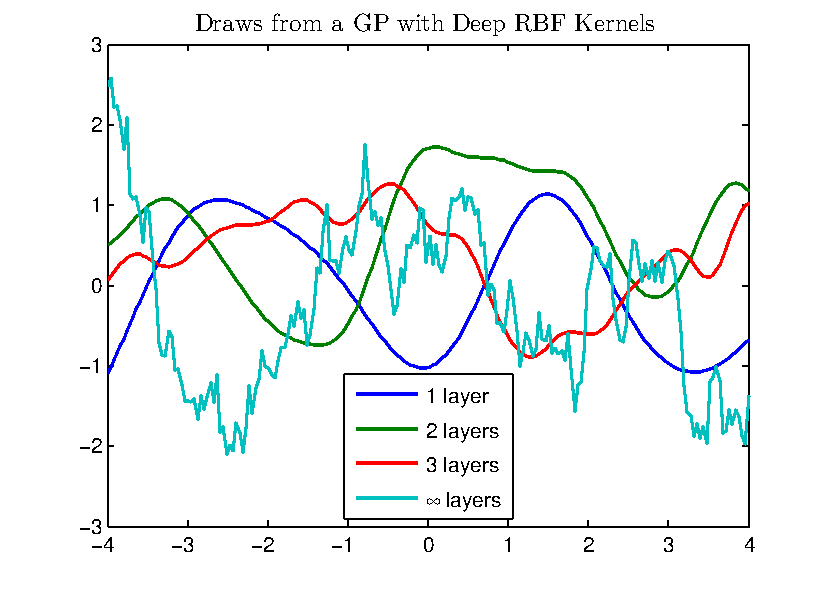
\includegraphics[width=\columnwidth, clip, trim = 0cm 0.1cm 0.9cm 0.35cm]{../figures/deep_kernel_connected_draws}
\end{tabular}
\end{centering}
\end{minipage}

\end{multicols}
\end{poster}
\end{document}
